\documentclass[10pt,journal,a4paper]{IEEEtran}
\usepackage[T1]{fontenc}
\usepackage{graphicx}
\usepackage{booktabs}
\usepackage{amsmath}
\usepackage{amssymb}
\usepackage{url}
\urlstyle{same}
\usepackage[hidelinks]{hyperref}

\begin{document}

\title{\vspace{-1.6em}\footnotesize\textsc{The University of Lahore $\bullet$ Department of Intelligent Systems $\bullet$ AI-101}\\[0.9em]
\Large Task A1: Breast Cancer Diagnosis from Cell-Nucleus Measurements}

\author{\normalsize Manaal Pervaiz \quad$\vert$\quad Roll No. 70173809 \quad$\vert$\quad Section BSES A\\
\normalsize Repository: \url{https://github.com/manaal6/AI101-ML-Assignment-70173809}\\
\normalsize Instructor: Dr. Muhammad Awais, AI Architect}
\date{}
\maketitle

\section{Introduction}
A fine-needle aspirate of a breast mass yields cell nuclei whose size, shape
and texture separate malignant from benign lesions. The diagnostic decision is
asymmetric: a missed malignancy can be fatal, while a false alarm costs only a
follow-up test. This report compares three classifiers on the Wisconsin
Diagnostic Breast Cancer (WDBC) data. The RBF SVM was best at the default
threshold (F1 0.963, ROC-AUC 0.993); lowering its threshold to 0.38 raised
malignant recall from 0.929 to 0.952 for a 0.024 precision cost, the operating
point a screening setting requires.

\section{Problem Statement}
Each example is a vector $x \in \mathbb{R}^{30}$ of nucleus measurements and the
label is $y \in \{0,1\}$, where $y=1$ denotes malignant. The task is supervised
binary classification. Success is measured by recall and F1 on the malignant
class and by ROC-AUC; accuracy is reported but is not the selection criterion
because the classes are unbalanced and the two errors have different costs.

\section{Dataset Used}
The Breast Cancer Wisconsin (Diagnostic) dataset, UCI Machine Learning
Repository id 17 \cite{uci}, is distributed with scikit-learn
\texttt{load\_breast\_cancer} \cite{sklearn}. It describes 569 digitised aspirates from the University of Wisconsin. Ten nucleus properties
(radius, texture, perimeter, area, smoothness, compactness, concavity, concave
points, symmetry, fractal dimension) are summarised by their mean, standard
error and ``worst'' value, giving 30 real-valued features \cite{street}. The
dataset has no missing values and no duplicate rows.

One preprocessing step is required. In scikit-learn, \texttt{target = 0} is
malignant and \texttt{target = 1} is benign; the labels were reversed so that
malignant is the positive class, which makes \texttt{predict\_proba(...)[:, 1]}
the malignant probability used by the threshold study. No rows or features were removed.

\section{Dataset Statistics}
Table~\ref{tab:stats} summarises the data and the stratified split. The classes
are moderately imbalanced (37.3\% malignant), so a constant ``benign'' predictor
already reaches 63.2\% accuracy on the test set.

\begin{table}[t]
\centering
\caption{Dataset statistics and split.}
\label{tab:stats}
\footnotesize
\setlength{\tabcolsep}{3pt}
\begin{tabular}{@{}ll@{}}
\toprule
Property & Value \\
\midrule
Samples & 569 \\
Features & 30 (10 properties $\times$ mean/SE/worst) \\
Malignant / benign & 212 (37.3\%) / 357 (62.7\%) \\
Missing values & 0 \\
Duplicate rows & 0 \\
Train / test & 455 / 114 \\
Malignant in train / test & 170 / 42 \\
\bottomrule
\end{tabular}
\end{table}

Figure~\ref{fig:corr} shows the correlation structure of the eleven mean
features. Fifteen feature pairs exceed $|r|=0.95$ and form two groups: the
size group (mean radius, perimeter and area, together with their worst-value
counterparts) and the error group (radius, perimeter and area error). Radius, perimeter and area restate one another; the redundancy is tested in
Section~VI.

\begin{figure}[t]
\centering
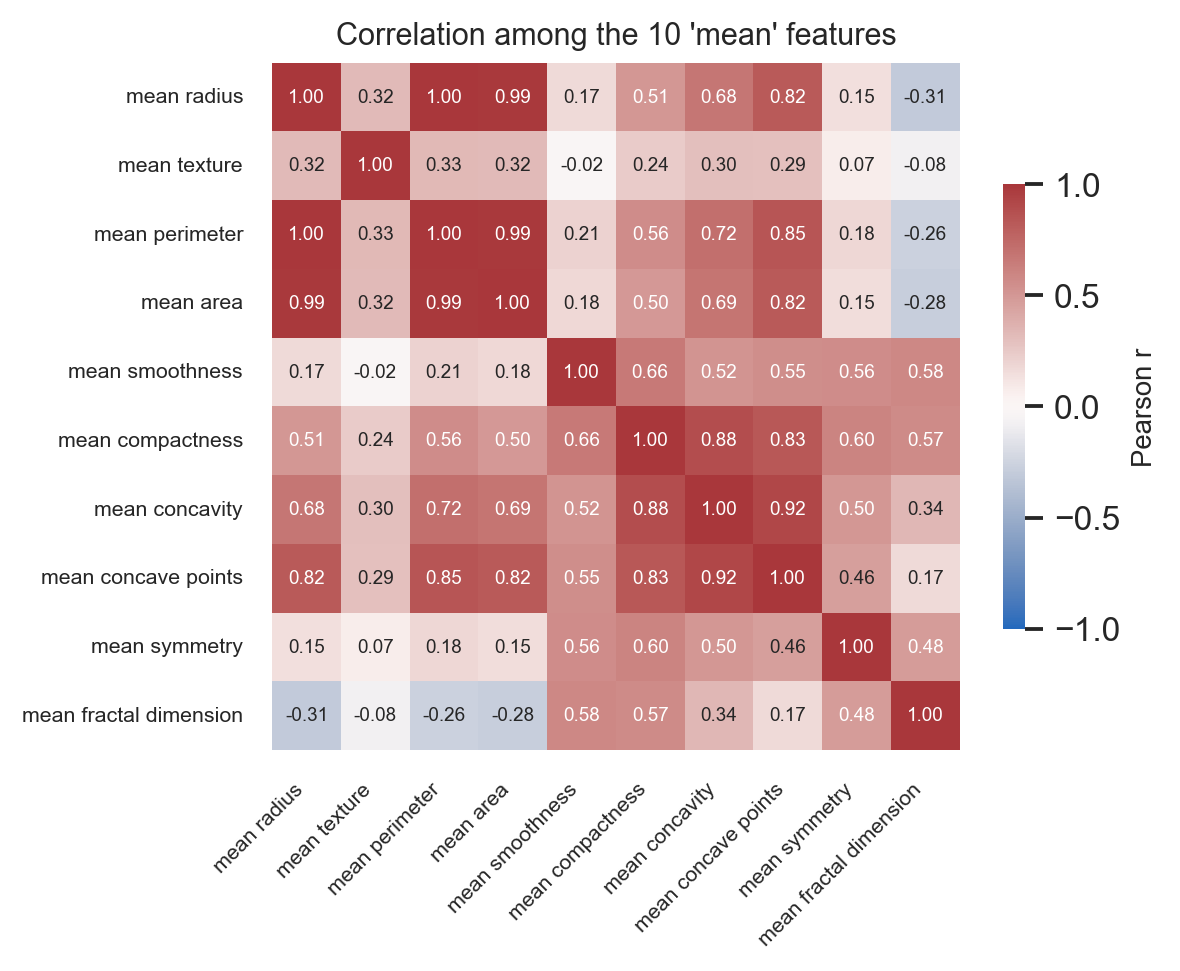
\includegraphics[width=0.94\columnwidth]{../figures/fig2b_correlation_mean_features.png}
\caption{Correlation heat-map of the mean nucleus features. Radius, perimeter
and area are almost collinear ($|r|>0.99$).}
\label{fig:corr}
\end{figure}

\section{Methodology}
\subsection{Learning Setting}
Three supervised classifiers are compared on the same 30 features:
Logistic Regression as a linear baseline whose coefficients are interpretable;
an SVM with an RBF kernel, which can represent a curved boundary with two
hyperparameters; and a Random Forest, which captures interactions and supplies
impurity-based feature importances. Every model is a scikit-learn
\texttt{Pipeline} of \texttt{StandardScaler} followed by the classifier, so
scaling is fitted inside each training fold and never on validation or test
data. All three use the same pipeline.

\subsection{Data Split Approach}
A stratified 80/20 split with seed 42 gives 455 training and 114 test samples,
preserving the malignant share (170 and 42). Hyperparameters are tuned with
5-fold stratified cross-validation on the training set only; the test set is
evaluated once, after all choices are frozen. The threshold is chosen from out-of-fold (OOF)
predictions, targeting recall 0.97 (the 0.95 floor plus a 0.02 margin); with 42
test malignancies, one case moves recall by 2.4 points. The ablation recomputes
correlations on the training split only.

\subsection{Parameter Settings}
Table~\ref{tab:params} lists the grids and the selected values. The search
minimises log-loss for the probabilistic models and uses the same folds
throughout; the Random Forest grid is smaller because each fit is much more
expensive.

\begin{table}[t]
\centering
\caption{Hyperparameter search (5-fold stratified CV) and selected values.}
\label{tab:params}
\footnotesize
\setlength{\tabcolsep}{2.5pt}
\begin{tabular}{@{}l p{3.6cm} l@{}}
\toprule
Model & Search space & Selected \\
\midrule
Logistic reg. & $C \in \{0.01,0.1,1,10,100\}$ & $C=1$ \\
SVM (RBF) & $C \in \{0.1,1,10,100\}$;\newline $\gamma \in \{\text{scale},0.01,0.001\}$ & $C=10$,\newline $\gamma=$ scale \\
Random forest & 200/400 trees; depth\newline $\{\text{None},10\}$; leaf $\{1,2\}$ & 200,\newline None, 1 \\
\bottomrule
\end{tabular}
\end{table}

\section{Results and Analysis}
\subsection{Results}
Table~\ref{tab:test} reports the single test-set evaluation; cross-validation
means are given in the text. The SVM is the best model on the primary metric
(F1 0.963) with perfect precision, while Logistic Regression has the highest
ROC-AUC (0.996). The Random Forest is slightly behind on recall (0.905) and
misses four malignancies.

\begin{table}[t]
\centering
\caption{Test-set results (114 samples, 42 malignant). Best per column in bold.}
\label{tab:test}
\footnotesize
\setlength{\tabcolsep}{3pt}
\begin{tabular}{@{}lccccc@{}}
\toprule
Model & Acc. & Prec. & Recall & F1 & ROC-AUC \\
\midrule
Logistic Reg. & 0.965 & 0.975 & 0.929 & 0.951 & \textbf{0.996} \\
SVM (RBF) & \textbf{0.974} & \textbf{1.000} & \textbf{0.929} & \textbf{0.963} & 0.993 \\
Random Forest & 0.965 & \textbf{1.000} & 0.905 & 0.950 & 0.994 \\
\bottomrule
\end{tabular}
\end{table}

Five-fold CV agrees with the test ranking: F1 is $0.964\pm0.021$ for Logistic
Regression, $0.967\pm0.011$ for the SVM and $0.949\pm0.021$ for the Random
Forest; ROC-AUC is $0.996\pm0.005$, $0.994\pm0.006$ and $0.989\pm0.007$. The
SVM also has the smallest fold-to-fold spread. Figure~\ref{fig:roc} shows the three ROC curves; all are close, and
the visible differences sit in the high-recall region that the threshold study
targets.

\begin{figure}[t]
\centering
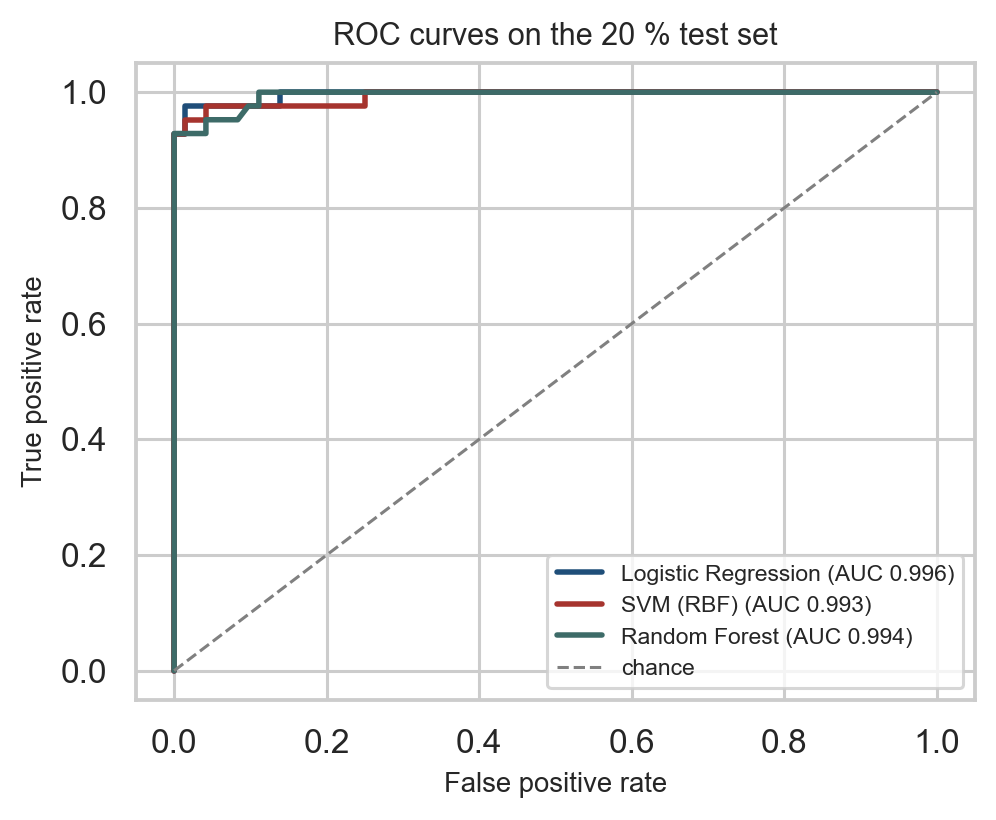
\includegraphics[width=0.95\columnwidth]{../figures/fig3_roc_curves.png}
\caption{ROC curves on the 114-sample test set. AUC: Logistic Regression 0.996,
SVM 0.993, Random Forest 0.994.}
\label{fig:roc}
\end{figure}

\subsection{Analysis}
\paragraph{Which model, and why accuracy misleads}
The SVM is the best choice: it matches the best recall, has perfect precision
and the most stable CV F1. Accuracy alone cannot show this. All three models sit
within one test case of each other (0.965--0.974), a spread of one sample, while
their false-negative counts differ by one (3, 3 and 4 of 42). A constant
``benign'' predictor scores 0.632 and catches no malignancy, and the SVM's
0.974 accuracy is 34 points higher, but that gap says nothing about the three
cancers it misses.

\paragraph{Threshold and error trade-off}
At the default 0.50 the SVM misses 3 of 42 malignancies with 0 false positives.
The OOF sweep finds that recall 0.97 is achievable only at $t=0.38$; the exact
0.95 boundary would be $t=0.68$. Applying $t=0.38$ to the test set raises recall
from 0.929 to 0.952 (40/42), lowers precision from 1.000 to 0.976 (one false
alarm), and leaves F1 at 0.964. The precision cost is 0.024, i.e.\ one extra benign
biopsy per 42 patients traded for one additional cancer found.

\paragraph{Which features matter, and does de-correlation hurt}
The Random Forest ranks worst perimeter (0.148), worst area (0.132), worst
concave points (0.110), mean concave points (0.088) and worst radius (0.085)
highest. The Logistic Regression coefficients agree on concavity and size but
also pick up worst texture (1.43) and radius error (1.23) as malignant-leaning,
and compactness error ($-0.91$) and fractal-dimension error ($-0.59$) as
benign-leaning. Dropping the seven features in the two correlated groups (23
features remain) leaves the SVM test F1 unchanged (0.963) and moves ROC-AUC by
$+0.0007$; LR is unchanged; the Random Forest loses 0.013 F1. The small
sample cannot resolve differences of that size, so the honest conclusion is that
the correlated features are harmless rather than necessary.

\paragraph{Limitations}
The test set has 42 malignant cases, so one case is 2.4 percentage points and
the ranking of close models is fragile. A single split was used and probabilities
were not calibrated. External validation is required before any clinical claim.

\section{Conclusion}
An RBF SVM on standardised nucleus features separates malignant from benign
masses with F1 0.963 and ROC-AUC 0.993, and a validation-chosen threshold of
0.38 buys the recall a screening setting needs at a 0.024 precision cost.
Dropping seven collinear size features changes nothing measurable. Next:
nested cross-validation, calibration, and explicit clinical utilities.

\section*{AI Use Disclosure}
I used opencode, an AI coding assistant, for notebook scaffolding, plotting code
and a first draft of this report's LaTeX. The following parts were generated or
substantially assisted by AI: the notebook's boilerplate cells and figure code,
and the report text, which I edited. I verified every number against the
executed notebook outputs and the saved result tables, re-ran the notebook from
top to bottom, and checked the code's leakage controls myself. All experiments,
results and the final analysis are produced and checked by me, and I take full
responsibility for this work.

\begin{thebibliography}{1}
\bibitem{street} W.~N. Street, W.~H. Wolberg and O.~L. Mangasarian, ``Nuclear
feature extraction for breast tumor diagnosis,'' \emph{Proc. IS\&T/SPIE
Symposium on Electronic Imaging}, vol.~1905, pp.~861--870, 1993.

\bibitem{uci} D.~Dua and C.~Graff, ``Breast Cancer Wisconsin (Diagnostic)
Data Set,'' UCI Machine Learning Repository, 2019.
\url{https://doi.org/10.24432/C5DW2B}.

\bibitem{sklearn} F.~Pedregosa \emph{et al.}, ``Scikit-learn: Machine learning
in Python,'' \emph{Journal of Machine Learning Research}, vol.~12,
pp.~2825--2830, 2011.

\bibitem{fawcett} T.~Fawcett, ``An introduction to ROC analysis,''
\emph{Pattern Recognition Letters}, vol.~27, no.~8, pp.~861--874, 2006.
\end{thebibliography}

\end{document}
